\documentclass[a4paper,12pt]{article}
\usepackage{indentfirst}
\usepackage[latin1,utf8]{inputenc}
\usepackage[portuges]{babel}
\usepackage[a4paper,portrait]{geometry}
\usepackage{amsmath} 
\usepackage{multicol}
\usepackage{makeidx} 
\usepackage{color} 
\usepackage{fancyhdr}
\usepackage{url}
\usepackage{lipsum} % for dummy text only
\usepackage[pdftex]{graphicx}
\usepackage{epstopdf}
\usepackage{graphics}
\usepackage{fancyhdr}
\usepackage{cleveref}
\usepackage{hyperref}
\usepackage{fixltx2e}
\usepackage{tabularx, booktabs}
\usepackage[utf8]{inputenc}
\usepackage{geometry}

%%%%%%%%%%% Predefinições de LaTeX do Tamanho da Página %%%%%%%%%%

\oddsidemargin = 30pt                    % Margem do lado esquerdo: 31pt
\topmargin = 18pt                        % Margem superior: 20pt  
\headheight = 12pt                       % Tamanho do 'header': 12pt 
\headsep = 25pt                          % Espaço entre o 'header' e o texto: 25pt
\textheight = 592pt                      % Altura do texto: 592pt
\textwidth = 390pt                       % Largura do texto: 390pt
\marginparsep = 10pt                     % Espaço entre margem esquerda e o texto: 10pt
\marginparwidth = 35pt                   % Margem esquerda: 35pt
\footskip = 20pt                         % Espaço entre o texto e o 'footer': 30pt

\hyphenation{asso-ciada}
\input epsf

\makeindex

\begin{document}
\renewcommand{\sfdefault}{lmss}
\renewcommand{\familydefault}{\sfdefault}
\fontfamily{lmss}\selectfont

\title{\bf Relatório de Sistemas Digitais \\
Traballho L2\\
Circuitos Combinatórios Típicos}
\author{João Oliveira\\
Tomás A. Reis\\
\\
Instituto Superior Técnico \\
Universidade de Lisboa}
\date{21 de Março de 2014 \\
Quinta-Feira LSD1}
\maketitle

\pagebreak
\section{Introdução}

\section{Projecto}

\subsection{Entradas e Saídas}
Estando A, B e S no intervalo [0;3] cada um será representado por dois bits, enquanto C\textsubscript{0} apenas necessitará de um. A codificação de A,B e S seguirão a conversão habitual de binário para decimal, como apresentado na seguintes tabela:


\subsection{Tabela de verdade}
 
\begin{table}[h]

\centering
\begin{tabular}{ || c  c | c c || c c| c || }
\hline
A\textsubscript{1} & A\textsubscript{0} & B\textsubscript{1} & B\textsubscript{0} & S\textsubscript{1} & S\textsubscript{0} & C\textsubscript{0} \\ \hline
0   & 0  & 0  & 0  & 0  & 0  & 0  \\ \hline
0   & 0  & 0  & 1  & 0  & 0  & 0  \\ \hline
0   & 0  & 1  & 0  & X  & X  & X  \\ \hline
0   &  0  & 1   & 1   & 0   & 0   & X   \\ \hline
0   &  1  &  0  & 0   & 0   & 0   & 1   \\ \hline
0   &  1  &  0  & 1   & 1   & 0   & 0   \\ \hline
0   &  1  &  1  & 0   & X   & X   & X   \\ \hline
0   &  1  &  1  & 1   & 0   & 1   & X   \\ \hline
1   &  0  &  0  & 0   & 0   & 1   & 0   \\ \hline
1   &  0  &  0  & 1   & 0   & 0   & 1   \\ \hline
1   &  0  &  1  & 0   & X   & X   & X   \\ \hline
1   &  0  &  1  & 1   & 1   & 0   & X   \\ \hline
1   &  1  &  0  & 0   & 0   & 1   & 1   \\ \hline
1   &  1  &  0  & 1   & 1   & 0   & 1   \\ \hline
1   &  1  &  1  & 0   & X   & X   & X   \\ \hline
1   &  1  &  1  & 1   & 1   & 1   & X   \\ \hline
\end{tabular}
\caption{Tabela de Verdade} % title of Table 
\end{table}

\subsection{Transformação das expressões algébricas}

\subsubsection{De forma a serem concretizadas com portas NAND-2, NAND-3 e NOT}
\begin{enumerate}
\item A partir da forma disjuntiva
\begin{equation}
\begin{split}
S_1(A_1,A_0,B_1,B_0) & = A_0\overline{B_1}B_0 + A_1B_1 \\
                     & = \overline{\overline{((A_0\overline{B_1}B_0)}
                         ~\overline {(A_1B_1))}}  \\  
\end{split}
\end{equation}
\begin{equation}
\begin{split}
C_0(A_1,A_0,B_1,B_0) & = A_0\overline{B_0} + A_1B_0 \\
                     & = \overline{\overline{((A_0 \overline{B_0})}
                         ~\overline{(A_1 B_0))}}  \\   
\end{split}
\end{equation}
Requisitos de implementação:
\begin{enumerate}
    \item 1x NAND-3
    \item 5x NAND-2
    \item 2x NOT
  \end{enumerate}


\subsection{Esquema Eléctrico}
Para a realização deste circuito segundo o logigrama previamente apresentado, 
serão necessários três circuitos integrados: um SN74LS10, com portas NAND-3,
e dois SN74LS00. De forma a necessitarmos apenas destes três CIs,
concretizaremos cada porta NOT juntando as entradas de uma porta NAND-2.
Isto é necessário pois precisamos de 5 portas NAND-2. Caso utilizássemos portas
NOT, a não ser que utilizássemos uma porta NAND-3 como NAND-2, utilizaríamos 
4 CIs, pois precisaríamos de dois SN74LS00 de qualquer forma;
porém considerámos mais simples a solução apresentada.

%\begin{figure}[h]
%\caption{Esquema Eléctrico}
%\begin{center}
%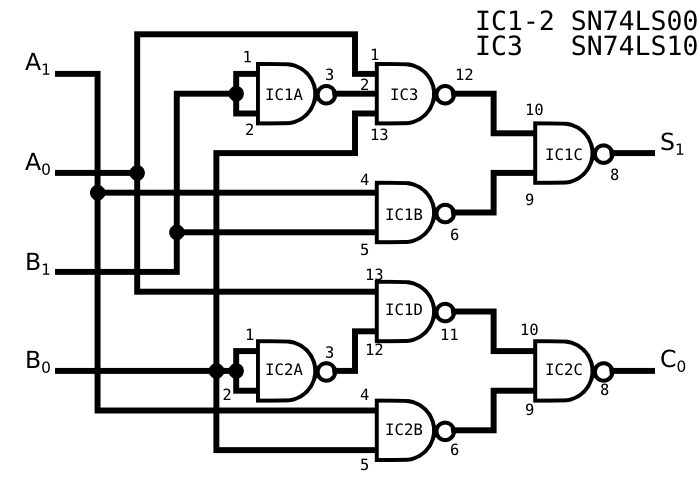
\includegraphics[scale=0.65]{SD_elect.png}
%\end{center}
%\end{figure}

\section{Montagem e Teste}
\subsection{Montagem}
Montou-se o circuito na {\it breadboard} utilizando os circuitos requisitados.
\subsection{Utilização da Ponta de Prova}
%\vspace*{10\baselineskip}
\pagebreak
\subsection{Teste do circuito}
\begin{table}
\centering
\begin{tabularx}{1.1\textwidth}{|| >{\setlength\hsize{1\hsize}\centering}X >{\setlength\hsize{1\hsize}\centering}X | >{\setlength\hsize{1\hsize}\centering}X >{\setlength\hsize{1\hsize}\centering}X || >{\setlength\hsize{1\hsize}\centering}X >{\setlength\hsize{1\hsize}\centering}X || >{\setlength\hsize{1\hsize}\centering}X  | c ||}
\hline 
\multicolumn{4}{||c||}{Valores de entrada} & \multicolumn{2}{c||}{Valores Esperados} & \multicolumn{2}{c||}{Valores de Saída} \\
  \hline
A\textsubscript{1} & A\textsubscript{0} & B\textsubscript{1} & B\textsubscript{0} & S\textsubscript{1} & C\textsubscript{0} & S\textsubscript{1} & C\textsubscript{0} \\ \hline
0   & 0  & 0  & 0  & L  & L && \\ \hline
0   & 0  & 0  & 1  & L  & L &&\\ \hline
0   & 0  & 1  & 0  & X  & X  &&\\ \hline
0   &  0  & 1   & 1   & L  & X &&\\ \hline
0   &  1  &  0  & 0   & L  & H  &&\\ \hline
0   &  1  &  0  & 1   & H  & L  &&\\ \hline
0   &  1  &  1  & 0   & X  & X  &&\\ \hline
0   &  1  &  1  & 1   & L  & X  &&\\ \hline
1   &  0  &  0  & 0   & L  & L  &&\\ \hline
1   &  0  &  0  & 1   & L  & H  &&\\ \hline
1   &  0  &  1  & 0   & X  & X  &&\\ \hline
1   &  0  &  1  & 1   & H  & X  &&\\ \hline
1   &  1  &  0  & 0   & L  & H  &&\\ \hline
1   &  1  &  0  & 1   & H  & H  &&\\ \hline
1   &  1  &  1  & 0   & X  & X  &&\\ \hline
1   &  1  &  1  & 1   & H  & X  &&\\ \hline
\end{tabularx}

\begin{table}
\centering
\begin{tabularx}{1.1\textwidth}{|| >{\setlength\hsize{1\hsize}\centering}X >{\setlength\hsize{1\hsize}\centering}X | >{\setlength\hsize{1\hsize}\centering}X >{\setlength\hsize{1\hsize}\centering}X || >{\setlength\hsize{1\hsize}\centering}X >{\setlength\hsize{1\hsize}\centering}X || >{\setlength\hsize{1\hsize}\centering}X  | c ||}
\hline 
\multicolumn{4}{||c||}{Valores de entrada} & \multicolumn{2}{c||}{Valores Esperados} & \multicolumn{2}{c||}{Valores Obtidos} \\
  \hline
a\textsubscript{3} & a\textsubscript{2} & a\textsubscript{1} & a\textsubscript{0} & f\textsubscript{1} & f\textsubscript{0} & f\textsubscript{1} & f\textsubscript{0} \\ \hline
0   & 0  & 0  & 0  & L  & L && \\ \hline
0   & 0  & 0  & 1  & L  & L &&\\ \hline
0   & 0  & 1  & 0  & X  & X  &&\\ \hline
0   &  0  & 1   & 1   & L  & X &&\\ \hline
0   &  1  &  0  & 0   & L  & H  &&\\ \hline
0   &  1  &  0  & 1   & H  & L  &&\\ \hline
0   &  1  &  1  & 0   & X  & X  &&\\ \hline
0   &  1  &  1  & 1   & L  & X  &&\\ \hline
1   &  0  &  0  & 0   & L  & L  &&\\ \hline
1   &  0  &  0  & 1   & L  & H  &&\\ \hline
1   &  0  &  1  & 0   & X  & X  &&\\ \hline
1   &  0  &  1  & 1   & H  & X  &&\\ \hline
1   &  1  &  0  & 0   & L  & H  &&\\ \hline
1   &  1  &  0  & 1   & H  & H  &&\\ \hline
1   &  1  &  1  & 0   & X  & X  &&\\ \hline
1   &  1  &  1  & 1   & H  & X  &&\\ \hline
\end{tabularx}
%\end{tabular} 
\caption{Tabela de Teste}
\end{table}
\vspace*{7\baselineskip}
\subsubsection{Comentário dos resultados}
%\vspace*{15\baselineskip}
\pagebreak
\section{Conclusão}
Com este trabalho teve-se como objectivo a concepção e concretização de um circuito que executa duas funções combinatórias. Para tal utilizou-se os Mapas de Karnaugh para obter as funções como soma de produtos e também como produto de somas para que depois fossem facilmente convertidas para expressões com, exclusivamente portas NAND e NOT ou NOR e NOT. A partir destas expressões escolhemos a mais económica e eficiente de implementar, tendo elaborado o respectivo diagrama lógico e esquema eléctrico após selecção dos circuitos integrados a usar.



\end{document}

-----------> footnotes
